The Design Process outlined in Section~\ref{design-process} developed five new prompt patterns to assist software architects in their decision-making process. These prompt patterns were tested in a hypothetical scenario within a CRM project at a startup. To address \textbf{\textit{RQ\textsubscript{3}}} and achieve our research goals, it is essential to incorporate the perspective of software architects in a real-world project. When considering the application of the prompt pattern sequence detailed in Section~\ref{pattern-based-prompt}, it is essential to analyze its effectiveness in supporting the decision-making process of architects, as well as its suitability and ease of implementation.

This chapter will present the study's findings from two companies where the prompt pattern sequence proposed in this study was implemented in distinct contexts: a financial institution and a pharmaceutical company. The primary focus will be to address the following research question:

\textbf{\textit{RQ\textsubscript{3}: What are the perceived benefits and challenges of using the proposed prompt sequence with generative AI tools in the architectural decision-making process from the perspective of software architects?}} -- This includes the opinions of software architects on real projects about the usefulness of generative AI information through prompt patterns sequence and its potential to streamline the decision-making process in their organizations.

Different systems were utilized in each of the two studies to apply the prompt patterns sequence and analyze the responses. The study comprises three main stages shown in Figure~\ref{keys-steps-study}. The initial stage involves gaining a general understanding of the selected system by making an architectural decision. In the subsequent stage, prompt patterns sequence is applied to provide decision-making information. Finally, software architects are requested to evaluate the information derived from the sequence of prompts. In each study, the steps are adjusted based on the complexity of the context. The primary technique employed for data collection was semi-structured interviews, and open analysis procedures were utilized to analyze the data based on the immediate results.

\begin{figure}[!ht]
    \centering
    \caption{\centering Keys Steps Study.}\label{keys-steps-study}
    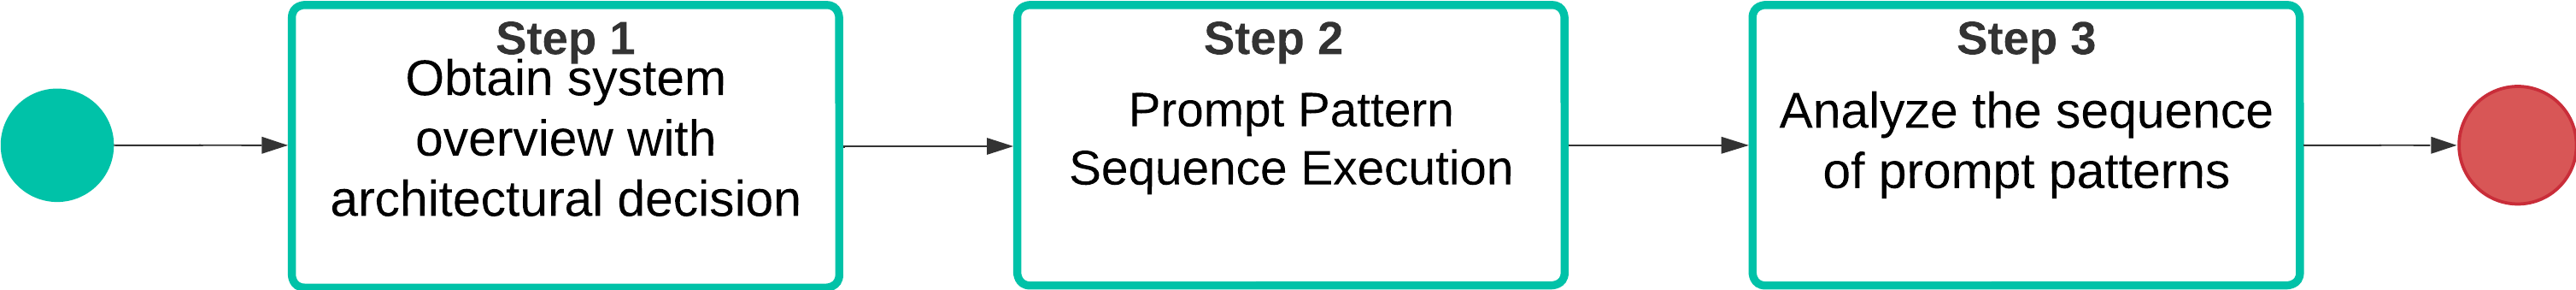
\includegraphics[width=1.0\textwidth]{figures/key-steps-scenario.png}
    \objectsource{\objectsourceauthor}
\end{figure}


\section{Research Methodology}
The methodology used in this work is different from traditional case studies and retrospective analyses in several significant ways~\cite{desouza2005experiences,runeson2012case}. Traditional case studies involve monitoring project activities or assignments in a real project setting to track specific attributes or establish relationships between different attributes~\cite{gustafsson2017single}. Retrospective studies involve reviewing completed projects or activities to capture lessons learned~\cite{hayes2011impact}. In contrast, this research actively involves software architects in a reflective and hypothetical evaluation of past decisions using AI-generated prompt patterns. 

Unlike traditional case studies, this approach goes beyond the observational nature of case studies by incorporating a speculative assessment of what could have happened if different information (i.e., the AI-generated prompts) had been available during decision-making~\cite{wohlin2003empirical}. Similarly, the work does not constitute a complete retrospective study, as its primary aim is not to derive lessons learned for future improvement. Instead, it aims to evaluate the hypothetical impact of AI-generated prompts on past decisions. 

This approach involves learning from the past and understanding how new technologies can influence decision-making processes. It is a unique combination of empirical research methods that utilize the strengths of case studies and retrospective analyses while overcoming their limitations through the innovative use of the Prompt Patterns Sequence in evaluating architectural decisions.

\MyParaBold{Design Process}

The study, which took place from October 2023 to March 2024, followed a methodology consisting of five distinct steps, as illustrated in Figure~\ref{industry-use-case}. It strategically recruited companies from various sectors to ensure diverse and widely applicable research findings. The selection of companies was guided by specific criteria such as industrial sector, size, complexity, and architectural challenges, laying a solid foundation for evaluating prompt pattern sequences in real-world scenarios.

\begin{figure}[!ht]
    \centering
    \caption{\centering Research Method Steps.}\label{industry-use-case}
    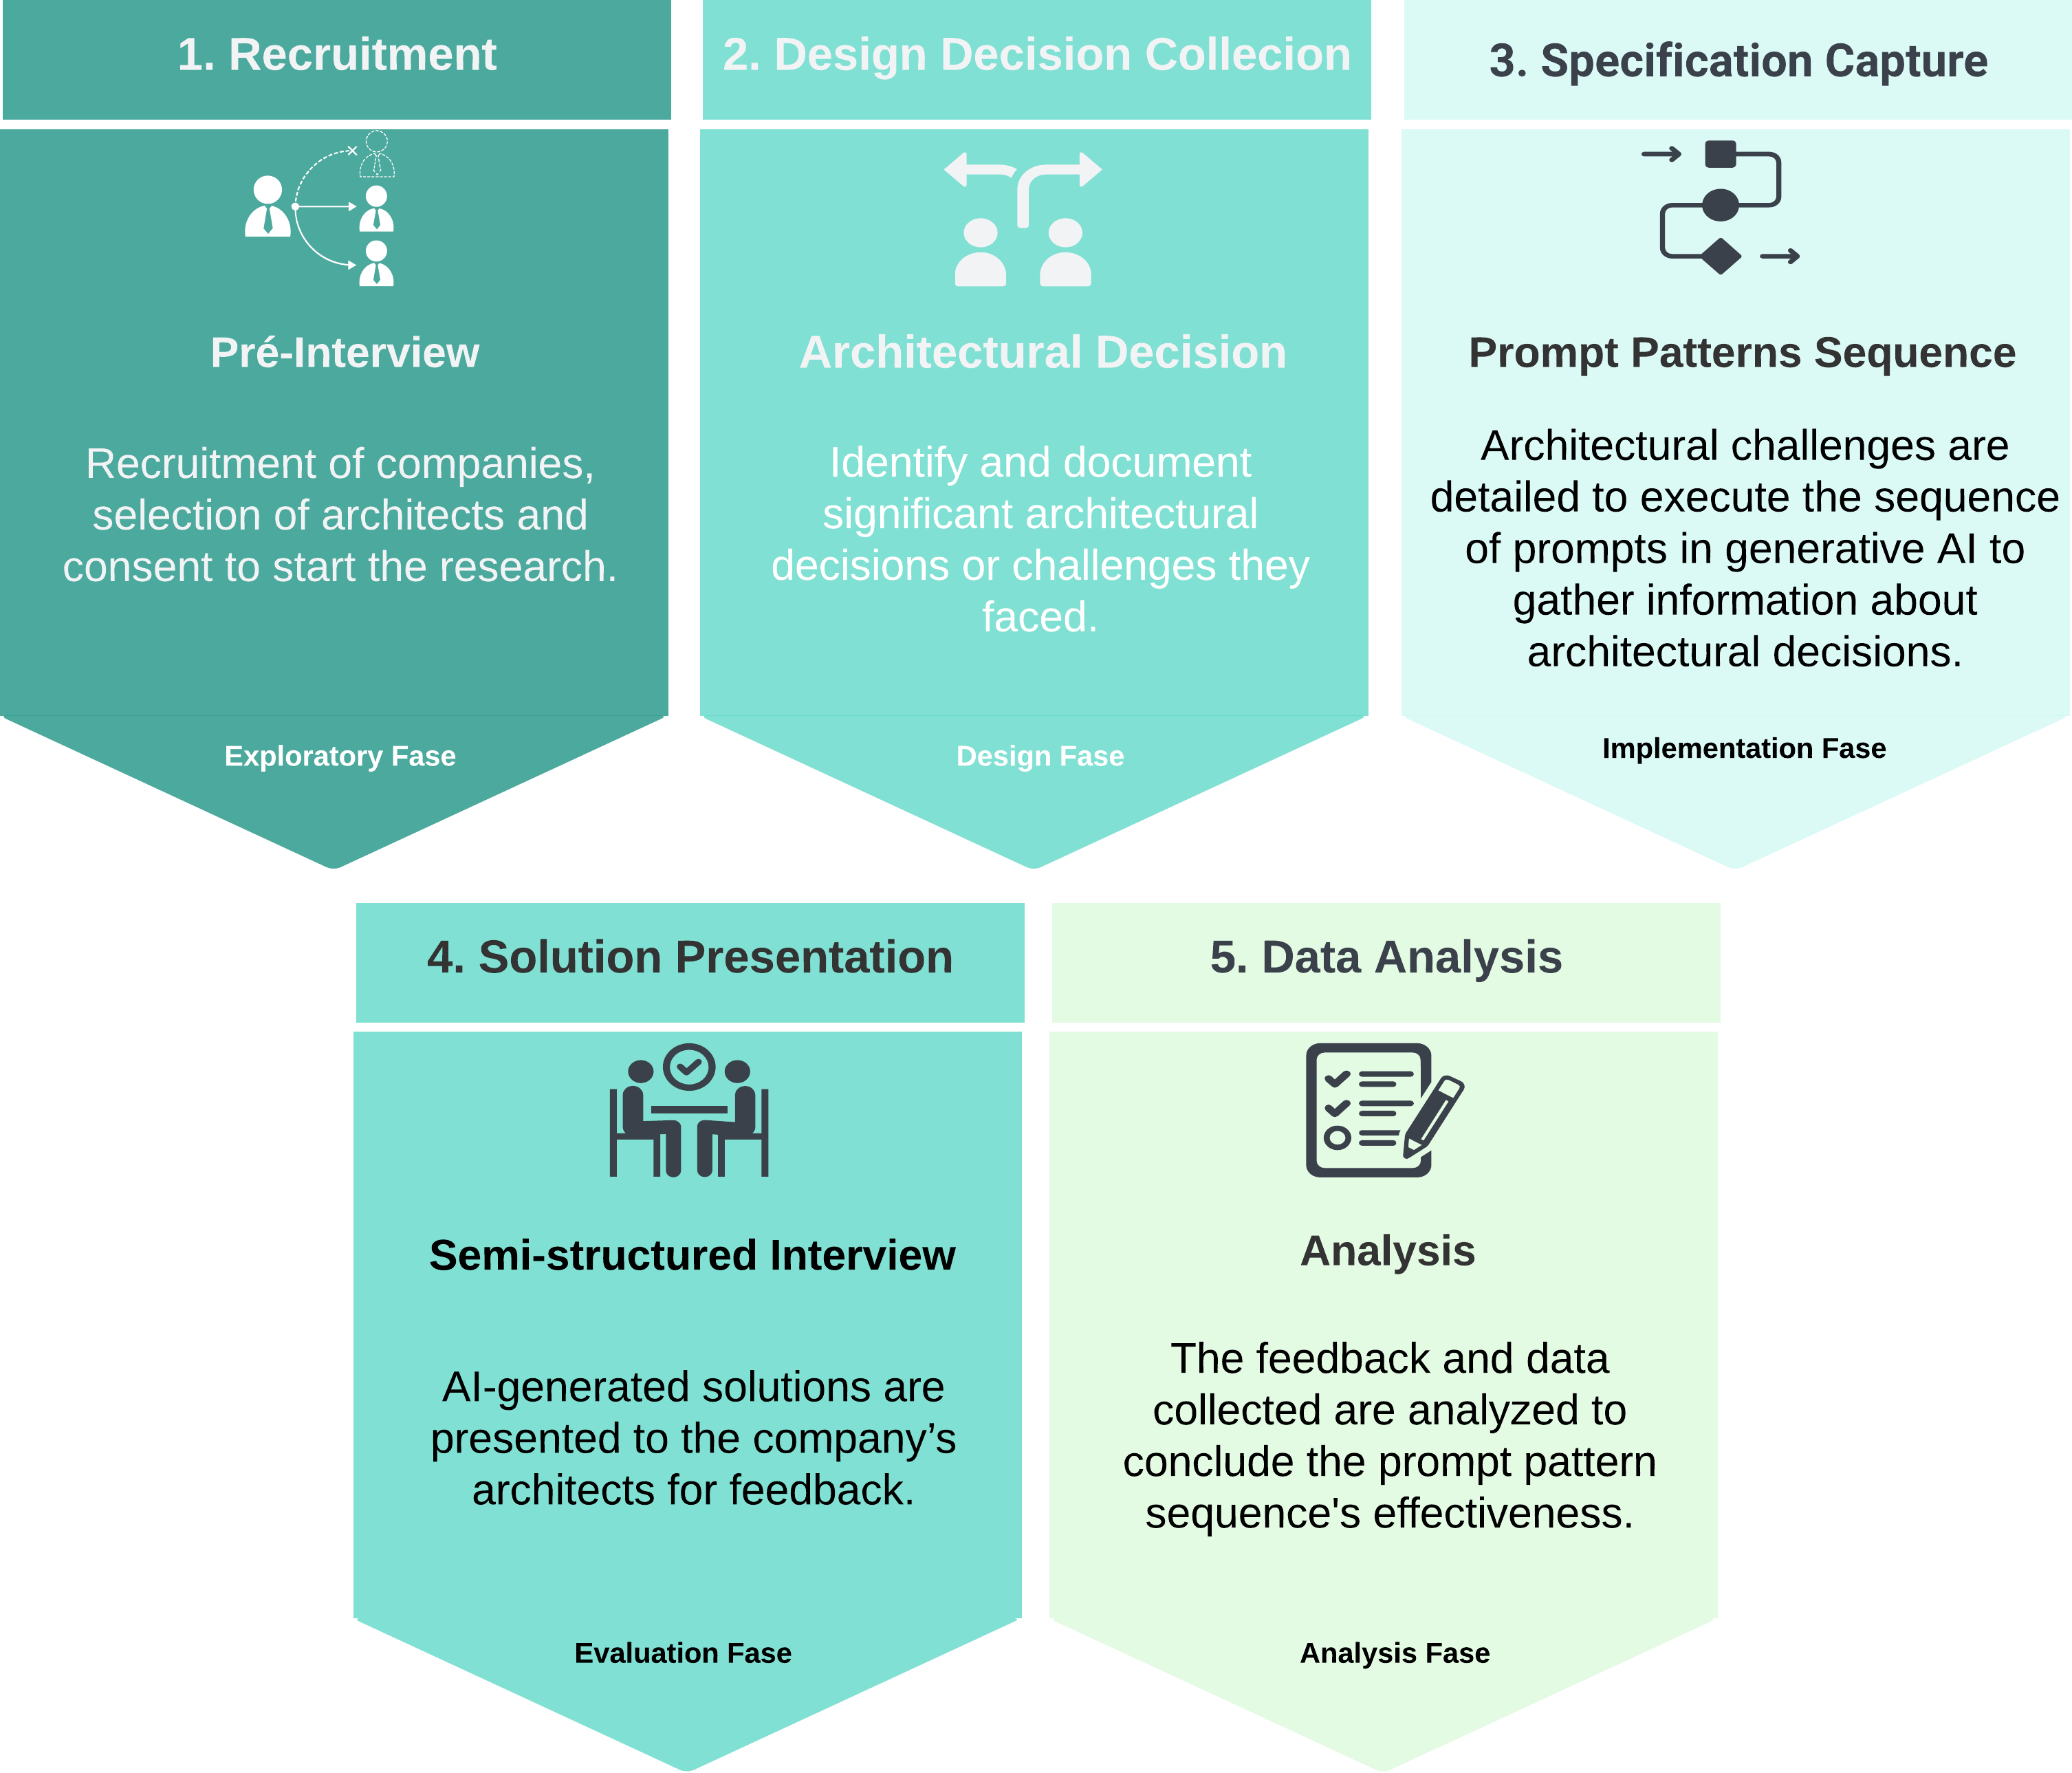
\includegraphics[width=1.0\textwidth]{figures/research-design-industry-use-cases.png}
    \objectsource{\objectsourceauthor}
\end{figure}

After recruiting the companies, the study focused on identifying significant architectural decisions and challenges within the chosen entities. Initial meetings were held with software architects from Company A(fictitious name for confidentiality reasons), a large Brazilian bank specializing in used car financing, and Company B(fictitious name for confidentiality reasons), a leading pharmacy chain with an extensive network. These engagements marked the formal start of the study, aiming to customize the application of AI tools to meet precise architectural requirements. The architects were selected based on their extensive experience, involvement in recent projects, and accessibility through professional networks, ensuring they could provide valuable insights into the deployability of AI-generated solutions.

The core of the study involved translating identified challenges into structured prompts for generative AI to capture the complexities of each company's architectural landscape. This process was enriched by interviews with team leader architects, which were meticulously recorded following an interview protocol outlined in Appendix~\ref{app:appendix_a}. The protocol encompassed questions about the architects' experience, their perceptions of the quality of AI responses, the sequence of prompt patterns, and their views on the utility of generative AI in their architectural decision-making processes.

Next, solutions derived from the Prompt Patterns Sequence were presented to the participating companies' architects for thorough evaluation. This phase provided a platform for assessing the practical relevance and utility of the AI-generated proposals, facilitated by the architects' openness to participate, sparked by the novel subject of generative AI.

The study culminated in a data analysis phase to synthesize the feedback and insights garnered throughout the investigation. The primary objective was to draw meaningful conclusions about the effectiveness of the prompt pattern sequence in aiding architectural decision-making. This final step significantly contributed to the discourse on AI integration in decision-making frameworks. It underscored the ethical considerations at the forefront of the study, ensuring confidentiality and anonymity for all participants.

\section{Real Scenario Financial Institution}

\MyParaBold{Company A - Change Track:}{Capture of safety and quality metrics.}

This project aims to determine the most influential architectural approach for capturing quality metrics, such as unit test coverage and security(security score), of software components for the company. This will be implemented within an automated change management process called Change Track, which aims to enable automatic deployment in productive environments.

\MyParaBold{Context:} Portal Tech is a web portal that creates and manages more than 18,000 software components, varying widely in technologies, languages, and frameworks. It communicates with continuous integration and continuous delivery (CI/CD) pipelines, using Jenkins for CI and Spinnaker and UrbanCode for CD. It is configured to integrate with specialized tools—SonarQube for code coverage and quality and Veracode for security—producing detailed reports for each creation of a RELEASE version.

However, a challenge arises when the current configuration only prevents a version from being released if code coverage is below 80\% or Veracode security metrics indicate severe criticism. Critical systems also require a more rigorous quality control and security level. Additionally, the change approval process remains manual, forcing analysts to consult each tool individually to evaluate quality and safety scores.

\MyParaBold{Proposal:} The Architecture team proposes centralizing quality and security reports in the Portal Tech, which will also record change requests. The idea is to eliminate manual analysis, allowing the change approval process to flow more efficiently and automatically.

\MyParaBold{Technical premises:} This integration must be carried out using Spring Boot, Apache Camel, and Spring Rest. The new code's client test coverage must exceed 80\%.

\MyParaBold{Uncertainties:}{The team responsible for exposing the security metrics APIs, Veracode, needed to make the API contract available so that we could carry out the integrations.}

\subsection{Applying Pattern-Based Prompt Sequence}
The section presents a hypothetical scenario to demonstrate the application of the pattern sequence. The scenario involves a startup developing a cloud-based CRM (Customer Relationship Management) system and facing an architectural decision challenge.

The following ideal sequence of prompt patterns will be used:
• 1st Software Architect Persona
• 2nd Technical Premises
• 3rd Uncertain Requirement Statement
• 4th Quality Attribute Question
• 5th Enterprise Architectural Context






\subsection{Analysis}

\section{Real Scenario Pharmaceutical Company}
\subsection{Applying Pattern-Based Prompt Sequence}
\subsection{Analysis}

\section{Discussion}

